
\chapter{\sf The Phase Field Crystal Model}\label{ch:pfc}

In this chapter, we first cover the general phase field models that preceded the PFC model. Then, the PFC model's free energy functional is derived from a first-principles theory of solidification, and its equilibrium properties are calculated. The phase diagram for the model is obtained. Finally, we define the dynamics of the model, including thermal fluctuations, and determine the conditions for different types of phase transitions to occur.

%%%%%%%%%%%%%%%%%%%%%%%%%%%%%%%%%%%%%%%%%%%%%%%%%%%%%%%%%%%%%%%%%%%%%%%%%%%%%%%%%%%%

\section{General phase field models}\label{sec:pfc_phasefield}

As the PFC model is a subclass of the general phase field models used in the study of phase transitions and interface motion, we give an overview of traditional phase field models. These concepts will be expanded upon in later sections describing the PFC model specifically.

A basic phase field model consists of a scalar field $\phi(\vec{x})$ (the phase field) representing a volume of material being simulated, along with a partial differential equation (PDE) governing the evolution of the phase field through time. The model also defines a free energy for its system in terms of the phase field, and the PDE drives the system towards its energy minima. More advanced models often incorporate multiple coupled fields, such as fields representing position-dependent temperature and solute concentration. Here we only consider single-field models for brevity.

The phase field in the models we consider here acts as an order parameter for the material being simulated: the field is zero in regions where the material is in a disordered phase, and nonzero in regions of ordered phase. For example, a pure material undergoing a phase transition from liquid to crystalline solid can be represented by a phase field corresponding to the density of the material relative to the liquid density, so that $\phi=0$ in the liquid and nonzero in the solid. Another example would be a mean-field Ising spin model where each spin can point in one of two directions, which could be simulated using a phase field model where $\phi$ is proportional to the average magnetization: $\phi=0$ in regions where the spin directions are completely random, and $|\phi|>0$ otherwise, with sign depending on the preferred spin direction. In these examples, the phase field is spatially constant within the bulk of regions with a specific order, and varies smoothly but rapidly at the interface between regions of different order.


For a given phase field model, the value $\phi$ takes in different phases, as well as the type of phase transition that the system undergoes, depends on the choice of local free energy density function $f(\phi,T)$. Here, $T$ is a temperature assumed to be constant over all space. This local free energy density accounts only for the energy in a bulk of constant $\phi$, neglecting interfacial energies between bulks of different $\phi$. Though the function $f$ can in general be an arbitrary function, we use the Landau theory of phase transitions to construct example polynomial forms for $f$ that can be tailored to different types of phase transitions.

Figure \ref{fig:landau_secondorder} plots a local energy density function that exhibits a second order phase transition, characterized by a continuous change of the order parameter as a critical temperature $T_c$ is passed. For $T>T_c$, the energy function has a single minimum at $\phi=0$ corresponding to the disordered phase, while for $T<T_c$ two minima of equal depths exist at nonzero values of $\phi$ corresponding to two ordered phases. The positions of these new minima move continuously from zero as $T$ decreases further from $T_c$. Such an energy function would be used for simulating spinodal decomposition in an Ising spin model with two spin orientations and no external field, or phase separation of two immiscible liquids such as oil and water.

Figure \ref{fig:landau_firstorder} plots a local energy density function that exhibits a first order phase transition, characterized by a discontinuous change of the order parameter as a critical temperature $T_c$ is passed. For $T>T_c$, the energy function's global minimum is at $\phi=0$ corresponding to the disordered phase, while for $T<T_c$ the global minimum has discontinuously moved to a value $\phi>0$ corresponding to an ordered phase. A local minimum exists at $\phi=0$ even for $T<T_c$, indicating the existence of a metastable disordered phase. Such an energy function would be appropriate for simulating solidification of a pure liquid into a solid through the process of nucleation.

\begin{figure}[h]
    \centering
\subfloat[]
{
    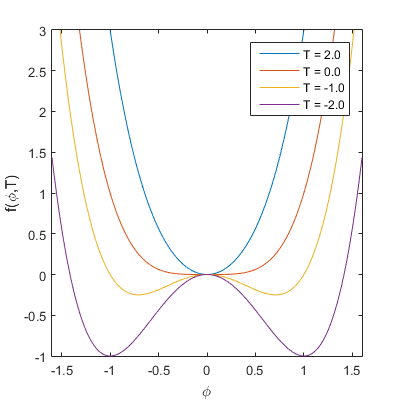
\includegraphics[width=0.5\textwidth]{fig_pfc/landau_secondorder}
    \label{fig:landau_secondorder}
}
\subfloat[]
{
    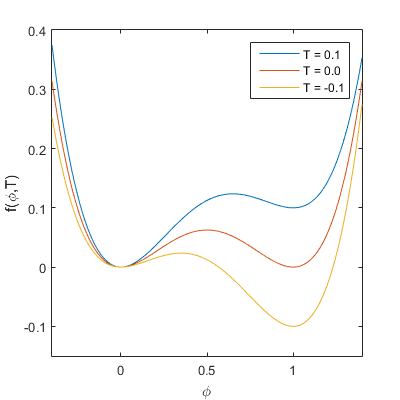
\includegraphics[width=0.5\textwidth]{fig_pfc/landau_firstorder}
    \label{fig:landau_firstorder}
}
    \caption{Plots of local energy density functions that lead to phase transitions at a critical temperature $T_c = 0$. The functions are (a) $f(\phi,T)=T\phi^2+\phi^4$ , (b) $f(\phi,T)=\phi^2(1-\phi)^2 + (3-2\phi)\phi^2T$}\label{fig:landau_functions}
\end{figure}



To evolve a phase field model's system through time, a description of the total energy is needed, including the contribution of interfaces between bulks of constant order parameter. This total energy is defined as a free energy functional $F[\phi]$ of the phase field. Systems consisting of bulk constant-field regions separated by thin interfaces, including the examples mentioned above, can be modeled using the free energy functional
%%
\begin{equation}\label{eq:ginzlandau}
F[\phi,T] = \int \left\{ \frac{1}{2} | W_o \nabla\phi |^2 + f(\phi(\vec{x}),T)  \right\}d\vec{x}
\end{equation}
%%
where the functional integral is over the volume of the system. The first term in the integral corresponds to an energy penalty for interfaces, and vanishes in bulks where the phase field is constant. The parameter $W_o$ determines how large the energy penalty for interfaces is. The term $f(\phi(\vec{x}),T)$ is the local free energy density discussed above. This functional is known as the Ginzburg-Landau free energy \cite{huang_statmech}.

The time-evolution PDE for a phase field model is chosen depending on whether the total phase field (i.e. the integral of the field over all space) is conserved. For example, the total phase field in an Ising model is not necessarily conserved, as there can be an arbitrary number of spins flipping to a new direction. Conversely, the spinodal decomposition of a mixture of immiscible liquids requires a conserved total phase field, assuming the total volume of each component liquid does not change. Nucleation of a solid from a pure liquid would also have conserved total field, due to conservation of mass. As our goal is to describe nucleation, we give here the PDE for a phase field model with conserved total field, which is
%%
\begin{equation}\label{eq:modelB}
\frac{\partial\phi}{\partial t}=M\nabla^2\frac{\delta F}{\delta \phi}
\end{equation}
%%
where $\frac{\delta F}{\delta \phi}$ is the functional derivative of $F[\phi]$, and $M$ is a solute mobility parameter. This PDE is known as the Cahn-Hilliard equation, or as Model B in condensed matter physics circles \cite{hohenberg77}. While we have introduced it in the context of traditional phase field methods, it will also be used in a later section for the PFC model. Figure \ref{fig:phasefield_spinodal} shows a system undergoing spinodal decomposition, simulated using the PDE of equation \ref{eq:modelB}, with the function $f(\phi,T)$ shown in figure \ref{fig:landau_secondorder} and with $T=-0.1$, $W_o=0.2$, and $M=1$.

\begin{figure}[!ht]
    \centering
\begin{tabular}{cccc}
\subfloat[]
{
    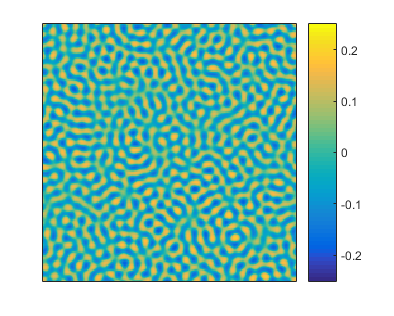
\includegraphics[width=0.5\textwidth]{fig_pfc/spinodal_5}
}
&\subfloat[]
{
    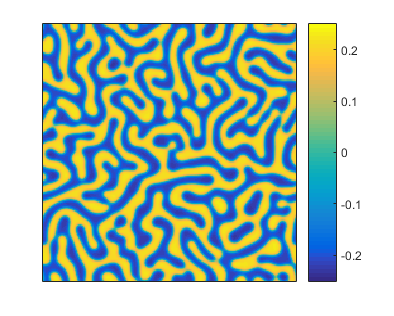
\includegraphics[width=0.5\textwidth]{fig_pfc/spinodal_10}
}\\
\subfloat[]
{
    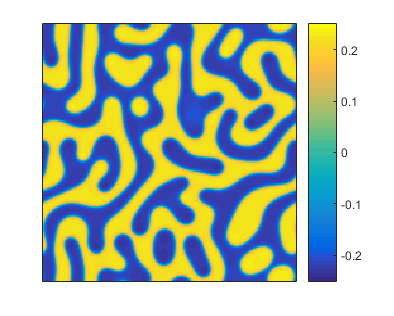
\includegraphics[width=0.5\textwidth]{fig_pfc/spinodal_40}
}
&\subfloat[]
{
    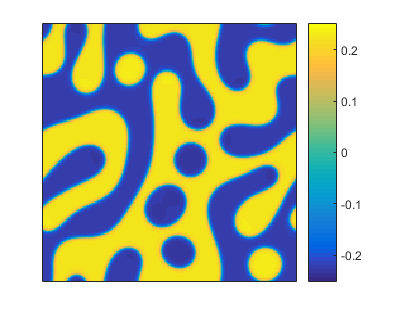
\includegraphics[width=0.5\textwidth]{fig_pfc/spinodal_200}
}
\end{tabular}
    \caption{Simulation of spinodal decomposition with a conserved total phase field, starting from a single disordered phase. The colors represent the phase field $\phi$. (a) to (d) are arranged in order of time, with initial disordered-only state not shown.}\label{fig:phasefield_spinodal}
\end{figure}

%%%%%%%%%%%%%%%%%%%%%%%%%%%%%%%%%%%%%%%%%%%%%%%%%%%%%%%%%%%%%%%%%%%%%%%%%%%%%%%%%%%%

\section{Deriving a free energy functional for PFC}\label{sec:pfc_deriv}

Instead of having a free energy functional that is minimized by bulk regions of constant phase field separated by thin interfaces, the PFC model's energy functional is minimized by a periodic phase field with a constant amplitude in the solid bulk and zero amplitude in the liquid bulk. The PFC model was originally defined as a phenomenological model built to reproduce certain atomic-scale structures and behaviors using a periodic phase field, following earlier work by Swift and Hohenberg \cite{hohenberg77-2} that derived a PDE exhibiting periodic pattern formation in convective systems. However, here we will instead derive the PFC model's free energy functional from classical density functional theory (CDFT) of solidification, and later obtain the PFC model's time-evolution PDE from this functional. The derivation presented below is for a two-dimensional system consisting of a single atomic specie capable of existing in a liquid phase and a solid phase, where the solid phase exhibits a triangular lattice structure. This derivation can be extended to allow a system in three dimensions, with more than one atomic specie, and with more complicated lattice structures \cites{provatas07,provatas_PFC,greenwood10,greenwood11,greenwood11_2}.

The CDFT used in the derivation, first proposed by Ramakrishnan and Yussouff \cite{ramakrishnan79}, provides as a starting point a Helmholtz free energy functional $\mathcal{F}[\rho]$ where $\rho(\vec{r})$ is the local number density of atoms in the system at position $\vec{r}$. Ramakrishnan and Yussouff obtain this free energy by expanding the full energy functional close to a reference liquid state in coexistence with a solid. Taking the reference liquid's density to be $\rho_o$ and defining $\delta\rho(\vec{r})=\rho(\vec{r})-\rho_o$, they show that
%%
\begin{equation}\label{eq:ramakF}
\frac{\mathcal{F}}{k_B T}= \int \left\{ \rho \ln\left(\frac{\rho}{\rho_o}\right)-\delta\rho \right\}d\vec{r} - \sum_{n=2}^{\infty} \frac{1}{n!} \int \prod_{i=1}^{n} d\vec{r}_i \delta\rho(\vec{r}_i)C_n(\vec{r}_1,\vec{r}_2,\vec{r}_3, ... ,\vec{r}_n)
\end{equation}
%%
where the integrals are over the volume of the system. $T$ is the temperature of the system, assumed to be constant through space, and $k_B$ is the Boltzmann constant. The functions $C_n$ are the $n$-point direct correlation functions of the liquid phase. The first approximation in this derivation is to truncate the integral series up to the two-point correlation function $C_2$. As the liquid phase is assumed to be isotropic, this correlation function can be simplified: $C_2(\vec{r}_1,\vec{r}_2)=C(|\vec{r}_1-\vec{r}_2|)$, where we have dropped the subscript for convenience. The truncated functional is then
%%
\begin{equation}\label{eq:ramakF_truncated}
\frac{\mathcal{F}}{k_B T}= \int \left\{ \rho \ln\left(\frac{\rho}{\rho_o}\right)-\delta\rho \right\}d\vec{r} - \frac{1}{2}\iint C(|\vec{r}_1-\vec{r}_2|)d\vec{r}_1 \delta\rho(\vec{r}_1)d\vec{r}_2 \delta\rho(\vec{r}_2)
\end{equation}
%%

\begin{figure}[h]
\centering
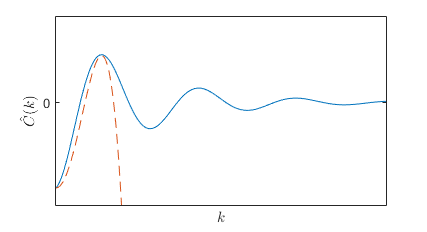
\includegraphics[width=0.8\textwidth]{fig_pfc/fourierCorrelation.png}
\caption{Sketch of the Fourier transform of the two-point direct correlation function. The solid curve is the full shape, the dashed curve is the approximated shape that includes only the first peak.}\label{fig:correlation_fourier}
\end{figure}

The next approximation is for the form of the correlation function $C$. In general, the Fourier transform $\hat{C}(k)$ of the two-point correlation function of a liquid formed of atoms that interact by the Lennard-Jones potential exhibits a rapidly decaying periodic shape \cite{mandel70}, due to the lack of long-range order. Figure \ref{fig:correlation_fourier} sketches the shape of such a function. We fit a polynomial function in Fourier space that matches only the first peak of the full function, approximating
%%
\begin{equation}\label{eq:correlationFourier}
\hat{C}(k) \approx -\hat{C}_0+\hat{C}_2 k^2 - \hat{C}_4 k^4
\end{equation}
%%
where $\hat{C}_0$, $\hat{C}_2$, and $\hat{C}_4$ are positive constants chosen so that the peaks match in position and height. The position of the peak in Fourier space determines the fundamental wavelength-scale of the resulting crystalline solid's reciprocal lattice. As there is only a single wavelength-scale, this approximate one-peak correlation function leads to a triangular lattice structure, the simplest two-dimensional Bravais lattice. A different choice for the correlation function can lead to more complex lattice symmetries \cite{greenwood10,greenwood11}. By calculating the position of the peak in Fourier space, we can obtain the real-space lattice constant $\alpha$ of the solid phase in terms of the constants appearing in equation \ref{eq:correlationFourier}, $\alpha = \sqrt[]{{2 \hat{C}_4}/{\hat{C}_2}}$, where we dropped a factor of $4\pi/\,\sqrt[]{3}$ for convenience. Taking the inverse Fourier transform of equation \ref{eq:correlationFourier} returns the correlation to real space giving
%%
\begin{equation}\label{eq:correlationReal}
C(|\vec{r}_1-\vec{r}_2|) \approx (-\hat{C}_0-\hat{C}_2 \nabla^2 - \hat{C}_4 \nabla^4)\delta(|\vec{r}_1-\vec{r}_2|)
\end{equation}
%%
where $\delta$ is the Dirac delta function.

Next, we define the dimensionless density field $n(\vec{r})=(\rho(\vec{r})-\rho_o)/\rho_o$ which will act as the phase field in our final derived energy functional. We also rescale the spatial variable by the lattice constant, $\vec{x} = \vec{r}/\alpha$. Plugging $n$ into equation \ref{eq:ramakF_truncated}, expanding the nonlinear term in the first integral to fourth order in $n$, and applying one integration on the correlation function obtained in equation \ref{eq:correlationReal} gives
%%
\begin{multline}\label{eq:derivedFunctional}
\frac{\mathcal{F}}{k_B T \rho_o \alpha^2}= \int d\vec{x}  \left\{2n + \frac{n^2}{2} - \frac{n^3}{6}+\frac{n^4}{12}\right\} \\ +\int d\vec{x}\left\{  -\frac{(n+1)^2}{2}(1-B^l+B^x)+ \frac{(n+1)}{2}B^x(2\nabla^2+\nabla^4)n \right\}
\end{multline}
%%
where we have defined $B^l=1+\rho_o \hat{C}_0$ and $B^x=\rho_o \hat{C}_2^2/4\hat{C}_4$. The final approximation of this derivation is to drop the terms in the integral of less than second order in $n$. This is done because constant terms and terms of first order in $n$ can only add a constant to the free energy functional: As $n$ is assumed to be a periodic function, integrating it over a volume much larger than the lattice constant $\alpha$ averages to a constant. We thus obtain the dimensionless free energy functional $F[n]$ used for the PFC model in all following sections,
%%
\begin{equation}\label{eq:PFC_energyFunctional}
F=\frac{\mathcal{F}}{k_B T \rho_o \alpha^2}= \int d\vec{x} \left\{ \frac{n^2}{2}B^l +\frac{n}{2}B^x(2\nabla^2+\nabla^4)n -t \frac{n^3}{3} + v \frac{n^4}{4}\right\}
\end{equation}
%%
where we have defined $t=1/2$ and $v=1/3$. The reason for these new parameters $t$ and $v$ is phenomenological: As the above derivation involved many crude approximations, it is expected that the resulting free energy functional might need to be tweaked under some circumstances to fit specific requirements. These parameters provide some degrees of freedom allowing such tweaking.

Define $\Delta B = B^l - B^x$. This quantity acts as the effective temperature of the derived PFC model. Returning to the definitions of $B^l$ and $B^x$ and to equation \ref{eq:correlationFourier}, we find that $\Delta B = 1 + \rho_o (\hat{C}_0-\hat{C}_2^2/\hat{C}_4)=1-\rho_o \hat{C}_m$ where $\hat{C}_m$ is the global maximum of the Fourier transformed two-point correlation function. If we fix $\rho_o$ while decreasing $\Delta B$, the peak of the correlation function increases, and vice versa. A higher peak in the correlation function $\hat{C}(k)$ indicates increased preference for the atoms to arrange themselves according to the solid phase's reciprocal lattice structure. Thus, decreasing $\Delta B$ is expected to trigger phase transition from liquid to solid, as will be seen in the following sections.




%%%%%%%%%%%%%%%%%%%%%%%%%%%%%%%%%%%%%%%%%%%%%%%%%%%%%%%%%%%%%%%%%%%%%%%%%%%%%%%%%%%%
\section{The one mode approximation}\label{sec:pfc_1mode}

As discussed in section \ref{sec:pfc_phasefield}, the phases and phase transitions in traditional phase field methods are determined by the local free energy density, a function of the order parameter. While the PFC model's dimensionless density field $n(\vec{x})$ does not act like a true order parameter in the way seen in that section, we can recover a pseudo-order parameter proportional to the amplitude of the periodic field $n$ by exploiting the periodicity to write a `one mode approximation' for $n$. This approximation then allows us to calculate the amplitude of the periodic field in the solid phase, as well as the dimensionless lattice constant of the solid phase.

Consider a system consisting of a single crystalline solid phase with no defects and a unique orientation. As the system is periodic, we can use reciprocal lattice theory to write
%%
\begin{equation}\label{eq:reciprocalLattice}
n(\vec{x}) = n_o + \sum_{\vec{G}} \phi_{\vec{G}} \cos(\vec{G} \cdot \vec{x})
\end{equation}
%%
where $n_o$ is the average of $n$ over the whole system, $\vec{G}$ are the reciprocal lattice vectors, and $\phi_{\vec{G}}$ are the corresponding amplitudes. The reciprocal lattice vectors can be expressed in two dimensions as $\vec{G}=\upsilon_1 \vec{q}_1+\upsilon_2 \vec{q}_2$ where $\vec{q}_i$ are the principle lattice vectors and $\upsilon_i$ are integers. For a triangular lattice in two dimensions, the principle reciprocal lattice vectors can be chosen as
%%
\begin{equation}\label{eq:principalRecVec}
\vec{q}_1 = -\frac{2}{\sqrt[]{3}}\cdot\frac{2\pi}{a}\left(\frac{\sqrt[]{3}}{2}\hat{x}+\frac{1}{2}\hat{y}\right), \qquad \vec{q}_2 = \frac{2}{\sqrt[]{3}}\cdot\frac{2\pi}{a}\hat{y}
\end{equation}
%%
where $a$ is the real-space lattice constant in dimensionless units, not to be confused with the dimensional lattice constant $\alpha$ used in the previous section.

The one mode approximation involves keeping only the terms in equation \ref{eq:reciprocalLattice} corresponding to the lowest order reciprocal lattice vectors. For a triangular lattice, these are the reciprocal lattice vectors for which $(\upsilon_1,\upsilon_2)\in \{(1,0),(0,1),(1,1)\}$. We then take the amplitudes $\phi_{\vec{G}}$ to all be equal, $\phi_{\vec{G}}=\phi/2$ for some parameter $\phi$. Applying the one mode approximation to equation \ref{eq:reciprocalLattice} and simplifying gives
%%
\begin{equation}\label{eq:oneMode}
n(x,y) = n_o + \phi\left(\frac{1}{2}\cos\left(\frac{4\pi}{\sqrt[]{3} a}y\right) - \cos\left(\frac{2\pi}{a}x\right)\cos\left(\frac{2\pi}{\sqrt[]{3} a}y\right) \right)
\end{equation}
%%

We then calculate the total free energy of the system by plugging equation \ref{eq:oneMode} into the free energy functional given by equation \ref{eq:PFC_energyFunctional}. Evaluating the resulting integral and minimizing the total free energy with respect to the lattice constant $a$ \cite{provatas_PFC}, we obtain that the energy is minimized for $a=4\pi/\,\sqrt[]{3}$ and is given in terms of the parameters $\phi$, $n_o$, $B^l$, and $B^x$ as
%%
\begin{multline}\label{eq:freeEnergy_minimized}
F(\phi, n_o, B^l, B^x) = B^l\frac{n_o^2}{2} -t\frac{n_o^3}{3}+v\frac{n_o^4}{4} \\ +\frac{3}{16}(\Delta B -n_o(2t-3vn_o))\phi^2 -\frac{1}{16}(t-3vn_o)\phi^3 + \frac{45v}{512}\phi^4
\end{multline}
%%

We find the locations of the minima of this energy function with respect to $\phi$ to be
%%
\begin{equation}\label{eq:freeEnergy_minima}
\phi_l=0 , \qquad \phi_s = \frac{4}{15v}\left(t-3 v n_o +\sqrt[]{t^2-15v\Delta B +12n_o v(2t-3vn_o)} \right)
\end{equation}
%%

The free energy function given in equation \ref{eq:freeEnergy_minimized} is analogous to the local free energy density function $f$ discussed in section \ref{sec:pfc_phasefield}: the parameter $\phi$ is the equivalent of the order parameters of traditional phase field models, while $\Delta B$ acts as an effective temperature. Figure \ref{fig:deltaB_wells} plots the free energy given by equation \ref{eq:freeEnergy_minimized} as a function of $\phi$ for different $\Delta B$, with fixed $n_o=0$. We observe the form of a free energy function that leads to a first-order transition between solid and liquid phases as $\Delta B$ decreases, with the minimum at $\phi=\phi_l=0$ corresponding to the liquid where the amplitude of the PFC model's periodic phase field $n$ is zero, and the minimum at $\phi=\phi_s>0$ corresponding to the solid where the amplitude is nonzero. Thus, by plugging equation \ref{eq:freeEnergy_minima} into equation \ref{eq:oneMode}, we predict that the value of the density field $n$ in the solid oscillates between $n_o+1.5\phi_s$ and $n_o-1.5\phi_s$.


\begin{figure}[h]
\centering
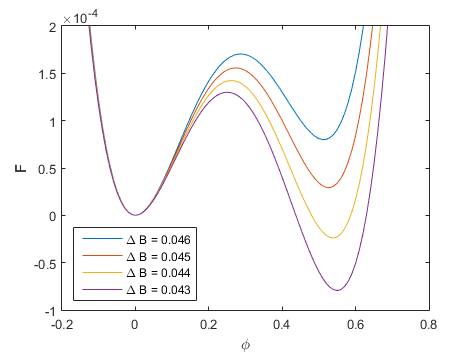
\includegraphics[width=0.8\textwidth]{fig_pfc/deltaBwells.png}
\caption{Free energy function for a single isolated phase, obtained through the one-mode approximation.}\label{fig:deltaB_wells}
\end{figure}




%%%%%%%%%%%%%%%%%%%%%%%%%%%%%%%%%%%%%%%%%%%%%%%%%%%%%%%%%%%%%%%%%%%%%%%%%%%%%%%%%%%%
\section{The PFC model's phase diagram}\label{sec:pfc_phasediag}


While we have approximated the free energy of a single isolated phase (equation \ref{eq:freeEnergy_minimized}) and described how it predicts a first-order phase transition as $\Delta B$ is varied, an actual simulated system can contain both liquid and solid phases in coexistence. Further, most physical materials are known to also transition from liquid to solid as the density is increased at fixed temperature. We will construct a phase diagram for our PFC model that depends on both the effective temperature $\Delta B$ and the average dimensionless density $n_o$, and includes areas of coexisting liquid and solid phases.

The usual method for determining the densities at which two phases coexist is to use the common tangent construction \cite{lupis_materials}. We first calculate the free energy curves of the solid and liquid phases in terms of $B^l$, $B^x$, and $n_o$. Setting $\phi=\phi_s$ in equation \ref{eq:freeEnergy_minimized} gives the free energy function $F_s$ for the solid phase in our model (not shown for brevity), and the free energy function $F_l$ for the liquid phase is obtained by setting $\phi=0$ in that equation, giving
%%
\begin{equation}\label{eq:freeEnergy_minimized_liquid}
F_l = B^l\frac{n_o^2}{2} -t\frac{n_o^3}{3}+v\frac{n_o^4}{4}
\end{equation}
%%

Then, fixing $B^l$ and $B^x$ to fix the effective temperature $\Delta B$, the free energies of the two coexisting phases are plotted as a function of average density $n_o$, and the common tangent to these two curves is found. Figure \ref{fig:commonTangent} plots the free energies of the liquid and solid phases as a function of $n_o$, at a fixed $\Delta B$, including the common tangent construction. Let $n_s$ and $n_l$ be the densities at which the common tangent intersects the energy curves of the solid and liquid phases respectively. For any density $n_o$ satisfying $n_l<n_o<n_s$, the system consists at equilibrium of coexisting phases, with average density $n_l$ for the liquid phase and $n_s$ for the solid phase. For densities where $n_o<n_l$ or $n_o>n_s$, the system at equilibrium consists fully of liquid or solid phase respectively. By repeating this construction for different $\Delta B$, we obtain the system's phase diagram as a function of $n_o$ and $\Delta B$. Figure \ref{fig:pfc_phasediag} displays part of the resulting phase diagram, including the `instability curve' defined later in section \ref{sec:pfc_phasetrans}.

\begin{figure}[h]
\centering
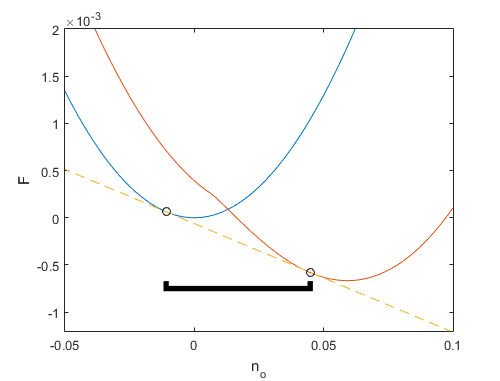
\includegraphics[width=0.8\textwidth]{fig_pfc/commonTangentMod.png}
\caption{The common tangent construction for $B^x=1$ and $B^l=1.055$. The energy function $F_l$ of the liquid phase is in blue, the energy function $F_s$ of the solid phase in red. The yellow line is the common tangent. The black circles are the points of intersection at densities $n_l$ (left) and $n_s$ (right). The black bar denotes the range of densities where the two phases coexist at equilibrium.  }\label{fig:commonTangent}
\end{figure}

\begin{figure}[h]
\centering
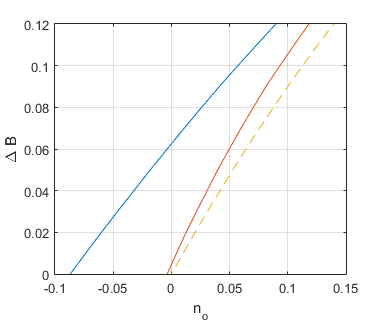
\includegraphics[width=0.8\textwidth]{fig_pfc/phaseDiagSpin.png}
\caption{Phase diagram of the PFC model, for $B^x=1$ fixed. The blue (red) curve is the locus of points $n_l$ ($n_s$) found through the common tangent construction, known as the `liquidus' (`solidus'). The yellow curve is the `instability curve'.}\label{fig:pfc_phasediag}
\end{figure}

%%%%%%%%%%%%%%%%%%%%%%%%%%%%%%%%%%%%%%%%%%%%%%%%%%%%%%%%%%%%%%%%%%%%%%%%%%%%%%%%%%%%
\section{The PFC model's dynamics}\label{sec:pfc_dynamics}

As the phase field of the PFC model represents an atomic density, the field must be conserved as the system is evolved. The time-evolution PDE of the model is thus the same as that of the traditional phase field Model B shown in equation \ref{eq:modelB}. We start with the PDE for the time-evolution of the dimensionful density $\rho(\vec{r})$ in terms of the free energy functional $\mathcal{F}$ of equation \ref{eq:ramakF_truncated},
%%
\begin{equation}\label{eq:pfc_dynamics_dimensionful}
\frac{\partial \rho}{\partial t} = M \nabla^2 \left(\frac{\delta \mathcal{F}}{\delta \rho}\right) + \nabla \cdot \vec\zeta
\end{equation}
%%
where $M$ is a solute mobility parameter and $\nabla \cdot \vec\zeta$ is a noise term representing thermal fluctuations that conserve the total field. $\vec\zeta=(\zeta_x(\vec{r},t),\zeta_y(\vec{r},t))$ is a two-component random vector field uncorrelated with itself in space and time, and satisfying the fluctuation-dissipation relation \cite{chaikin_condensed,sancho_noise}, expressed as
%%
\begin{equation}\label{eq:pfc_noise_dimensionful}
\langle \zeta_i(\vec{r},t),\zeta_j(\vec{r}\,',t') \rangle = -2 k_B T M \delta(\vec{r}-\vec{r}\,')\delta(t-t')\delta_{ij}
\end{equation}
%%
where $T$ is the temperature, $k_B$ is the Boltzmann constant, $\delta(\cdot)$ is the Dirac delta function, and $\delta_{ij}$ is the Kronecker delta function. Equation \ref{eq:pfc_noise_dimensionful} is to be interpreted as specifying that each $\zeta_i$ is a random variable uncorrelated with itself and follows a Gaussian distribution with standard deviation $\sigma = \sqrt[]{2k_B T M}$.

To obtain the time-evolution PDE corresponding to our dimensionless free energy functional $F=\mathcal{F}/k_B T \rho_o \alpha^2$ of equation \ref{eq:PFC_energyFunctional}, we again set $n=(\rho-\rho_o)/\rho_o$ and $\vec{x}=\vec{r}/\alpha$, giving
%%
\begin{equation}\label{eq:pfc_dynamics_dimensionless}
\frac{\partial n}{\partial t} = \Gamma \nabla^2 \left(\frac{\delta F}{\delta n}\right) + \nabla \cdot \vec\xi
\end{equation}
%%
where $\Gamma = k_B T M/\rho_o $ and the dimensionless noise term satisfies
%%
\begin{equation}\label{eq:pfc_noise_dimensionless}
\langle \xi_i(\vec{x},t),\xi_j(\vec{x}\,',t') \rangle = - N_a^2 \delta(\vec{x}-\vec{x}\,')\delta(t-t')\delta_{ij}
\end{equation}
%%
for $N_a^2=2\Gamma/\rho_o \alpha^2$ \cite{kocher16}. Evaluating the functional derivative in equation \ref{eq:pfc_dynamics_dimensionless} gives the time-evolution PDE for the dimensionless density $n(\vec{x})$, written as
%%
\begin{equation}\label{eq:pfc_dynamics_dimensionless_final}
\frac{\partial n}{\partial t} = \Gamma \nabla^2 \left[(B^l +B^x (2\nabla^2+\nabla^4))n -tn^2+vn^3\right] + \nabla \cdot \vec\xi
\end{equation}
%%

What remains is to specify the value of the dimensionless noise standard deviation, $N_a$. While one could attempt to match it to a specific real material's values of $\rho_o$ and $\alpha$, it has been shown by Kocher, Ofori-Opoku, and Provatas \cite{kocher16} that $N_a$ must be chosen as a function of the PFC model's $B^l$ and $B^x$ parameters to ensure proper behavior of capillary fluctuations. These authors also show that a cutoff must be applied to the noise's spectrum: noise modes with wavenumber $k>2\pi/a$ in Fourier space must be set to zero, where $a$ is the dimensionless lattice constant. This cutoff can be understood as eliminating unphysical fluctuations on scales smaller than the lattice separation, as these fluctuations would have already been accounted for in obtaining the CDFT used in section \ref{sec:pfc_deriv} to derive the PFC model's free energy functional. It can also be understood from a numerical perspective \cite{plapp11}: not implementing such a cutoff causes the atomic-scale dynamics of the simulated model to strongly depend on the discretization scheme used, due to more noise modes being available for a finer grid discretization.

Though we have scaled out the dimensional temperature from equation \ref{eq:pfc_noise_dimensionless}, we require that the steady probability distribution of states of our system continue obeying the Boltzmann distribution. To ensure this, the fluctuation-dissipation theorem must again be obeyed \cite{sancho_noise} by defining a fluctuation temperature $T_{r}$ through $N_a^2\approx 2\Gamma T_{r}$. The relation is only approximate due to the cutoff applied to the noise's Fourier modes, and the Boltzmann constant $k_B$ is assumed to be included in $T_r$. In this work, we assume that $T_{r}$ is used in calculating values related to the fluctuation-driven dynamics of the system, such as the Boltzmann factor $\exp(-E/T_r)$ that gives the probability of a state of energy $E$ relative to the probability of a state of zero energy. This fluctuation temperature should not be confused with either the dimensional $T$ that was scaled out of the PFC model's equations, or $\Delta B$ which is normally considered the model's effective temperature due to its previously-detailed role in determining the phase diagram. While $\Delta B$ and $T_{r}$ are effectively coupled by following the recommended values of $N_a$ from \cite{kocher16}, care should be taken when using these separate values in equations that require a temperature value or dependence. 

%It should be noted that the choice of noise standard deviation $N_a$ in equation \ref{eq:pfc_noise_dimensionless} also defines a fluctuation temperature $T_{r}$ for the model, due again to the fluctuation-dissipation relation $N_a^2\approx 2T_{r}$. 

%%%%%%%%%%%%%%%%%%%%%%%%%%%%%%%%%%%%%%%%%%%%%%%%%%%%%%%%%%%%%%%%%%%%%%%%%%%%%%%%%%%%
\section{Types of phase transitions in the PFC model}\label{sec:pfc_phasetrans}

Returning to figure \ref{fig:deltaB_wells}, we note that even when the global minimum of the effective free energy density function is at $\phi=\phi_s>0$, a local minimum remains at $\phi=\phi_l=0$. The existence of this metastable energy well indicates that the system does not necessarily spontaneously undergo a phase transition when a decrease in $\Delta B$ places it below the liquidus line of its phase diagram. Depending on how far a system consisting only of liquid is `undercooled' (that is, how far $\Delta B$ is instantaneously decreased below the liquidus), one of two kinetic paths can lead to phase transition: either nucleation or spinodal decomposition \cite{chaikin_condensed,provatas_PFC}.

Nucleation occurs when an energy barrier exists between the liquid and solid phases despite the solid phase being more energetically favorable. The liquid phase then resides in a metastable well of the energy function. This situation occurs for a relatively small drop of $\Delta B$ below the liquidus, and in such a case the phase transition is triggered stochastically in localized areas of the system when and where thermal fluctuations manage to push the local energy density out of the metastable well. The newly formed `nucleus' of solid then expands into the surrounding liquid until equilibrium is reached. Figure \ref{fig:pfc_example_nucleation} shows a PFC simulation undergoing nucleation.

\begin{figure}[h]
    \centering
\subfloat[]
{
    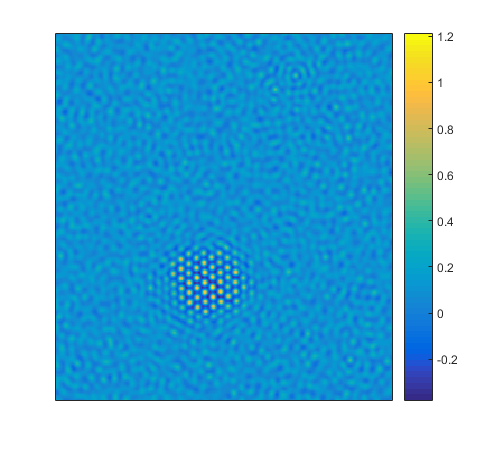
\includegraphics[width=0.5\textwidth]{fig_pfc/pfc_nuc1}
}
\subfloat[]
{
    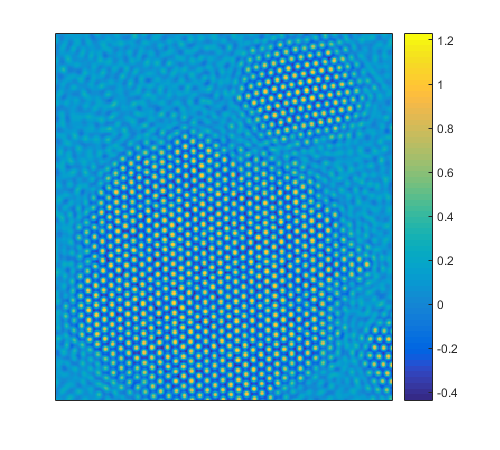
\includegraphics[width=0.5\textwidth]{fig_pfc/pfc_nuc2}
}
    \caption{Nucleation in a PFC simulation. Images ordered by simulation time elapsed. Parameters chosen were $B^x=1.00$, $B^l=1.10$, $n_o=0.1$, and $N_a=0.2$. (a) a solid nucleus appears in the middle of liquid phase (at simulation time $t=750$), (b) the first nucleus grows while other nuclei continue appearing (at $t=1250$).}\label{fig:pfc_example_nucleation}
\end{figure}

Conversely, for a large drop of $\Delta B$, the energy barrier between liquid and solid phases disappears. This leads to the system undergoing phase transition spontaneously and at all points in space simultaneously, as it decomposes spinodally into a ratio of solid and liquid volume predicted by the phase diagram at that point of parameter space. Figure \ref{fig:pfc_example_spinodal} shows a PFC simulation undergoing spinodal decomposition, without the need for thermal fluctuations.

\begin{figure}[h]
    \centering
\subfloat[]
{
    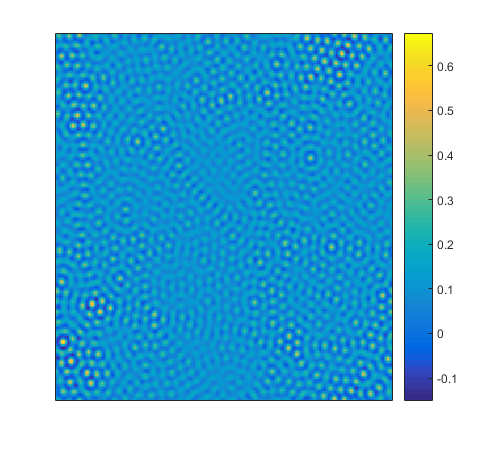
\includegraphics[width=0.5\textwidth]{fig_pfc/pfc_spi1}
}
\subfloat[]
{
    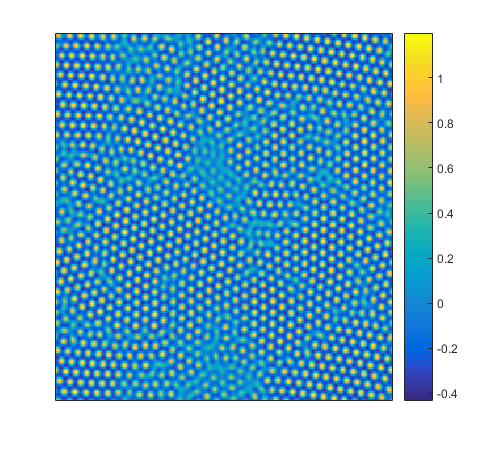
\includegraphics[width=0.5\textwidth]{fig_pfc/pfc_spi3}
}
    \caption{Spinodal decomposition in a PFC simulation. Images ordered by simulation time elapsed. Parameters chosen were $B^x=1.00$, $B^l=1.08$, $n_o=0.1$, and $N_a=0$. Numerical noise on the order of $10^{-7}$ was included in the initial state of the system, to break the initial symmetry. }\label{fig:pfc_example_spinodal}
\end{figure}

The precise $\Delta B$ at which behavior changes from nucleation-based phase transition to spinodal decomposition can be determined by calculating the linear stability of the phase field with respect to fluctuations. We do so by considering a perturbation from the liquid state,
%%
\begin{equation}\label{eq:perturb_n}
n(\vec{x},t) = n_o + \delta n(\vec{x},t)
\end{equation}
%%
where $\delta n(\vec{x},t)$ is the perturbation. Substituting this into equation \ref{eq:pfc_dynamics_dimensionless_final}, neglecting the noise term, and isolating the terms of order $\delta n$ gives
%%
\begin{equation}
\begin{split}
\frac{\partial \delta n}{\partial t} &= \Gamma \nabla^2 \left(B^x (2\nabla^2+\nabla^4)\delta n +g'(n_o)\delta n \right)\\ &= \Gamma \nabla^2 \left(B^x (2\nabla^2+\nabla^4) + B^l-2tn_o+3vn_o^2 \right)\delta n
\end{split}
\end{equation}
%%
where we have defined $g(n)=B^l n -tn^2 +vn^3$ and then Taylor expanded $g(n_o+\delta n)$ to order $\delta n$. Transforming the above to Fourier space gives
%%
\begin{equation}\label{eq:perturb_n_dynamics_fourier}
\frac{\partial \delta \hat{n}_k}{\partial t} =  -\Gamma k^2 \left(B^x (-2k^2+k^4) + B^l-2tn_o+3vn_o^2 \right)\delta \hat{n}_k
\end{equation}
%%

Equation \ref{eq:perturb_n_dynamics_fourier} is a first order ordinary differential equation with solution
%%
\begin{equation}\label{eq:perturn_ode_sol}
\begin{split}
\delta\hat{n}_k(t) &= \exp\left\{-\Gamma k^2 \left(B^x (-2k^2+k^4) + B^l-2tn_o+3vn_o^2 \right)t\right\} \delta\hat{n}_k(t=0)\\&\equiv e^{\gamma_k t}\, \delta\hat{n}_k(t=0)
\end{split}
\end{equation}
%%
for the defined coefficient $\gamma_k$. We see that, when no other fluctuations are present, the $k$th Fourier mode of the perturbation $\delta n$ will grow if and only if $\gamma_k > 0$. Taking the parameter $\Gamma$ to be positive (as it is a dimensionless solute mobility parameter), we find that having $\gamma_k > 0$ for some non-empty subset of available $k$ modes requires
%%
\begin{equation}\label{eq:pfc_spinodal_requirement}
\Delta B < 2tn_o -3vn_o^2
\end{equation}
%%

Although not all $k$ modes will be unstable to perturbation for a given set of parameters satisfying equation \ref{eq:pfc_spinodal_requirement}, having a non-empty subset of these modes be unstable is sufficient for the system to be unstable as a whole, since the nonlinear nature of the PFC model's time-evolution PDE ensures that any fluctuation will eventually spread to all $k$ modes due to nonlinear mode coupling. Equation \ref{eq:pfc_spinodal_requirement} thus gives the region of the PFC's phase diagram where an arbitrarily small fluctuation from the liquid state will always grow, resulting in phase transition. This is a characteristic of spinodal decomposition, where there exists no energy barrier between the liquid and solid phases. The remaining region of the phase diagram requires nucleation for any phase transition to take place. We refer to the boundary between the nucleating and non-nucleating regions as the instability curve.

For the remainder of this thesis, we will focus only on nucleation. Any simulated PFC system will have parameters chosen such that the system is above its instability curve.







